% !Mode:: "TeX:UTF-8"
% !TEX program  = xelatex

\section{Construction}




\subsection{Jetson Nano环境搭建}
待完成

\subsection{Model Training}

%此部分主要介绍了在不同的数据集上使用不同的backbone网络+FaPN进行训练,并评估了在数据集的测试集上的性能。

In this section, I mainly introduce the training process of different backbone networks with FaPN on different datasets and evaluates the performance on the test set of the dataset.

\textbf{COCO 2017 Dataset: }MS COCO \cite{lin2014microsoft} consists of over 100K images with different objects and annotations including bounding boxes and segmentation masks. I use the train2017 set (about 118K images) for training and report the results val2017 set (5K images) for comparison. For both object detection and instance segmentation tasks, there are 80 categories; for panoptic segmentation tasks, there are 80 stuff and 53 stuff classes annotated.


\begin{table}[htb]
	% h-here,t-top,b-bottom,优先级依次下降
		\begin{center}
		% 居中
			\caption{Notations}\label{Notation}
			\begin{tabular}{|c|l|} % 三线表不能有竖线,l-left,c-center,r-right
				\toprule
				\textbf{Notation} & \textbf{Definition}\\
				\hline
				$f_a(·)$ & feature aligned procedure\\
				$f_s(·)$ & feature selection procedure\\
				$f_m(·)$ & feature importance modeling procedure\\
				$P^u_i$ & unaligned feature i in upsampled layer\\
				$\textbf{z}$ & importance value set\\
				$\Delta_i$ & offset distance\\
				$C_i$ & unaligned feature i\\
				$H$ & height of the feature map\\
				$W$ & width of the feature map\\
				$x_\textbf{p}$ & feature in the given position p\\
				$\Delta\textbf{p}_n$&tuple of the additional offset\\
				$f_i$&aligned feature i\\
				$AP$&average precision\\
				\bottomrule
			\end{tabular}
		\end{center}
	\end{table}

The deformable convolution is used in the feature aligned procedure. It can be mathematically presented as Equation(\ref{con:deformableConvolution}).



\begin{equation}
    \begin{aligned}
    \hat{x}_\textbf{p}= \sum_{n = 1}^{N}w_n * x_{\textbf{p}+\textbf{p}_n},
    \label{con:deformableConvolution}
    \end{aligned}
\end{equation}

input $\textbf{c}_i \in \mathbb{R}^{H_i * W_i}$ is the feature map and the conv layer with $k * k$. The output $\hat{x}_\textbf{p}$ is the feature in the given position $\textbf{p}$. Then it can be calculated according to the sum of the convolution procedure. However, for the FAM module, the additional offset distance is added, so the Equation(4) can be reformulated as Equation(\ref{con:famConvolution}).

\begin{equation}
    \begin{aligned}
    \hat{x}_\textbf{p}= \sum_{n = 1}^{N}w_n * x_{\textbf{p}+\textbf{p}_n+\Delta\textbf{p}_n},
    \label{con:famConvolution}
    \end{aligned}
\end{equation}

where the $\Delta\textbf{p}_n$ is a tuple $[h, w] \in [(-H_i, H_i), (-W_i, W_i)]$.

\begin{algorithm}[htbp]
	\caption{Pseudo-Code of Feature Aligned Module} 
	\label{alg1} 
	\begin{algorithmic}
		\REQUIRE 
        The input channel, $C_{in}$;
		\ The output channel, $C_{out}$;
		\ The bottom-up feature map, $f_m$;
		\ The top-down feature map, $f_t$;
		\ENSURE 
        The aligned feature, $\hat{f}_i$;
		\STATE Execute the FSM module with $C_{in}$ and $C_{out}$.
		\STATE Initialize the offset layer with nn.Conv2d.
		\STATE Use nn.Relu as the activation function.
		\IF{$f_m$'s size not equals to the size of $f_t$}
        \STATE Use F.interpolate to upsample the $f_t$.
		\ENDIF 
		\STATE Select important features $\hat{f}_t$ through FSM module.
		\STATE $\hat{f}_i \gets \hat{f}_t + f_m$.

	\end{algorithmic} 
\end{algorithm}

\begin{algorithm}[htbp]
	\caption{Pseudo-Code of Feature Selection Module} 
	\label{alg2} 
	\begin{algorithmic}
		\REQUIRE 
        The input channel, $C_{in}$;
		\ The output channel, $C_{out}$;
		\ENSURE The selected feature, $\hat{f}_i$;
		\STATE Use F.avg\_pool2d to get the result of average pool of input feature map.
		\STATE Use nn.Conv2d to get the feature vector $\textbf{z} =  [z_1, z_2, ..., z_D]$.
		\STATE Multiply the $\textbf{z}$ with input feature map, get the result $x$.
		\STATE $C_{out} \gets nn.Conv2d(C_{in}, C_{out}, 1, x)$. 

	\end{algorithmic} 
\end{algorithm}


FaPN adds feature selection module \cite{hu2018squeeze} and feature aligned module based on FPN. Compared with FPN, Instance Segmentation has achieved 1.2\%-2.6\% improvement \cite{huang2021fapn}. The FaPN-based modules in this paper are all trained on the COCO2017 dataset in the aforementioned backbone networks. The training parameters are presented in the relevant environment for the training and running section.


For the performance evaluation of the above-mentioned models, Average Precision, that is, the AP value is the main evaluation index. The AP value can be divided into $AP_s$, $AP_m$, and $AP_l$ according to the size of the detection target; $AP_s$, $AP_m$, and $AP_l$ respectively represent small, medium and large The detection effect of objects. mIoU, also known as mean Intersection-over-Union, is mainly used to evaluate the performance of semantic segmentation \cite{padilla2021comparative}.

%miou,两框交集/两框并集
$$ mIoU = \frac{1}{k+1} \sum_{i=0}^{k}\frac{p_{ii}}{\sum_{i=0}^{k}p_{ij}+\sum_{j=0}^{k}p_{ji}-p_{ii}}$$

$$AP = \frac{1}{N}\sum_{n=1}^{N}Pr_{interp}(R_r(n))\ $$
$$AP_s = AP (small\ objects\ that\ area < 32^2)$$
$$AP_m = AP (medium\ objects\ that\ 32^2 < area < 96^2)$$
$$AP_l = AP (large\ objects\ that\ area > 96^2)$$

\begin{figure}[htb]
    \centering
    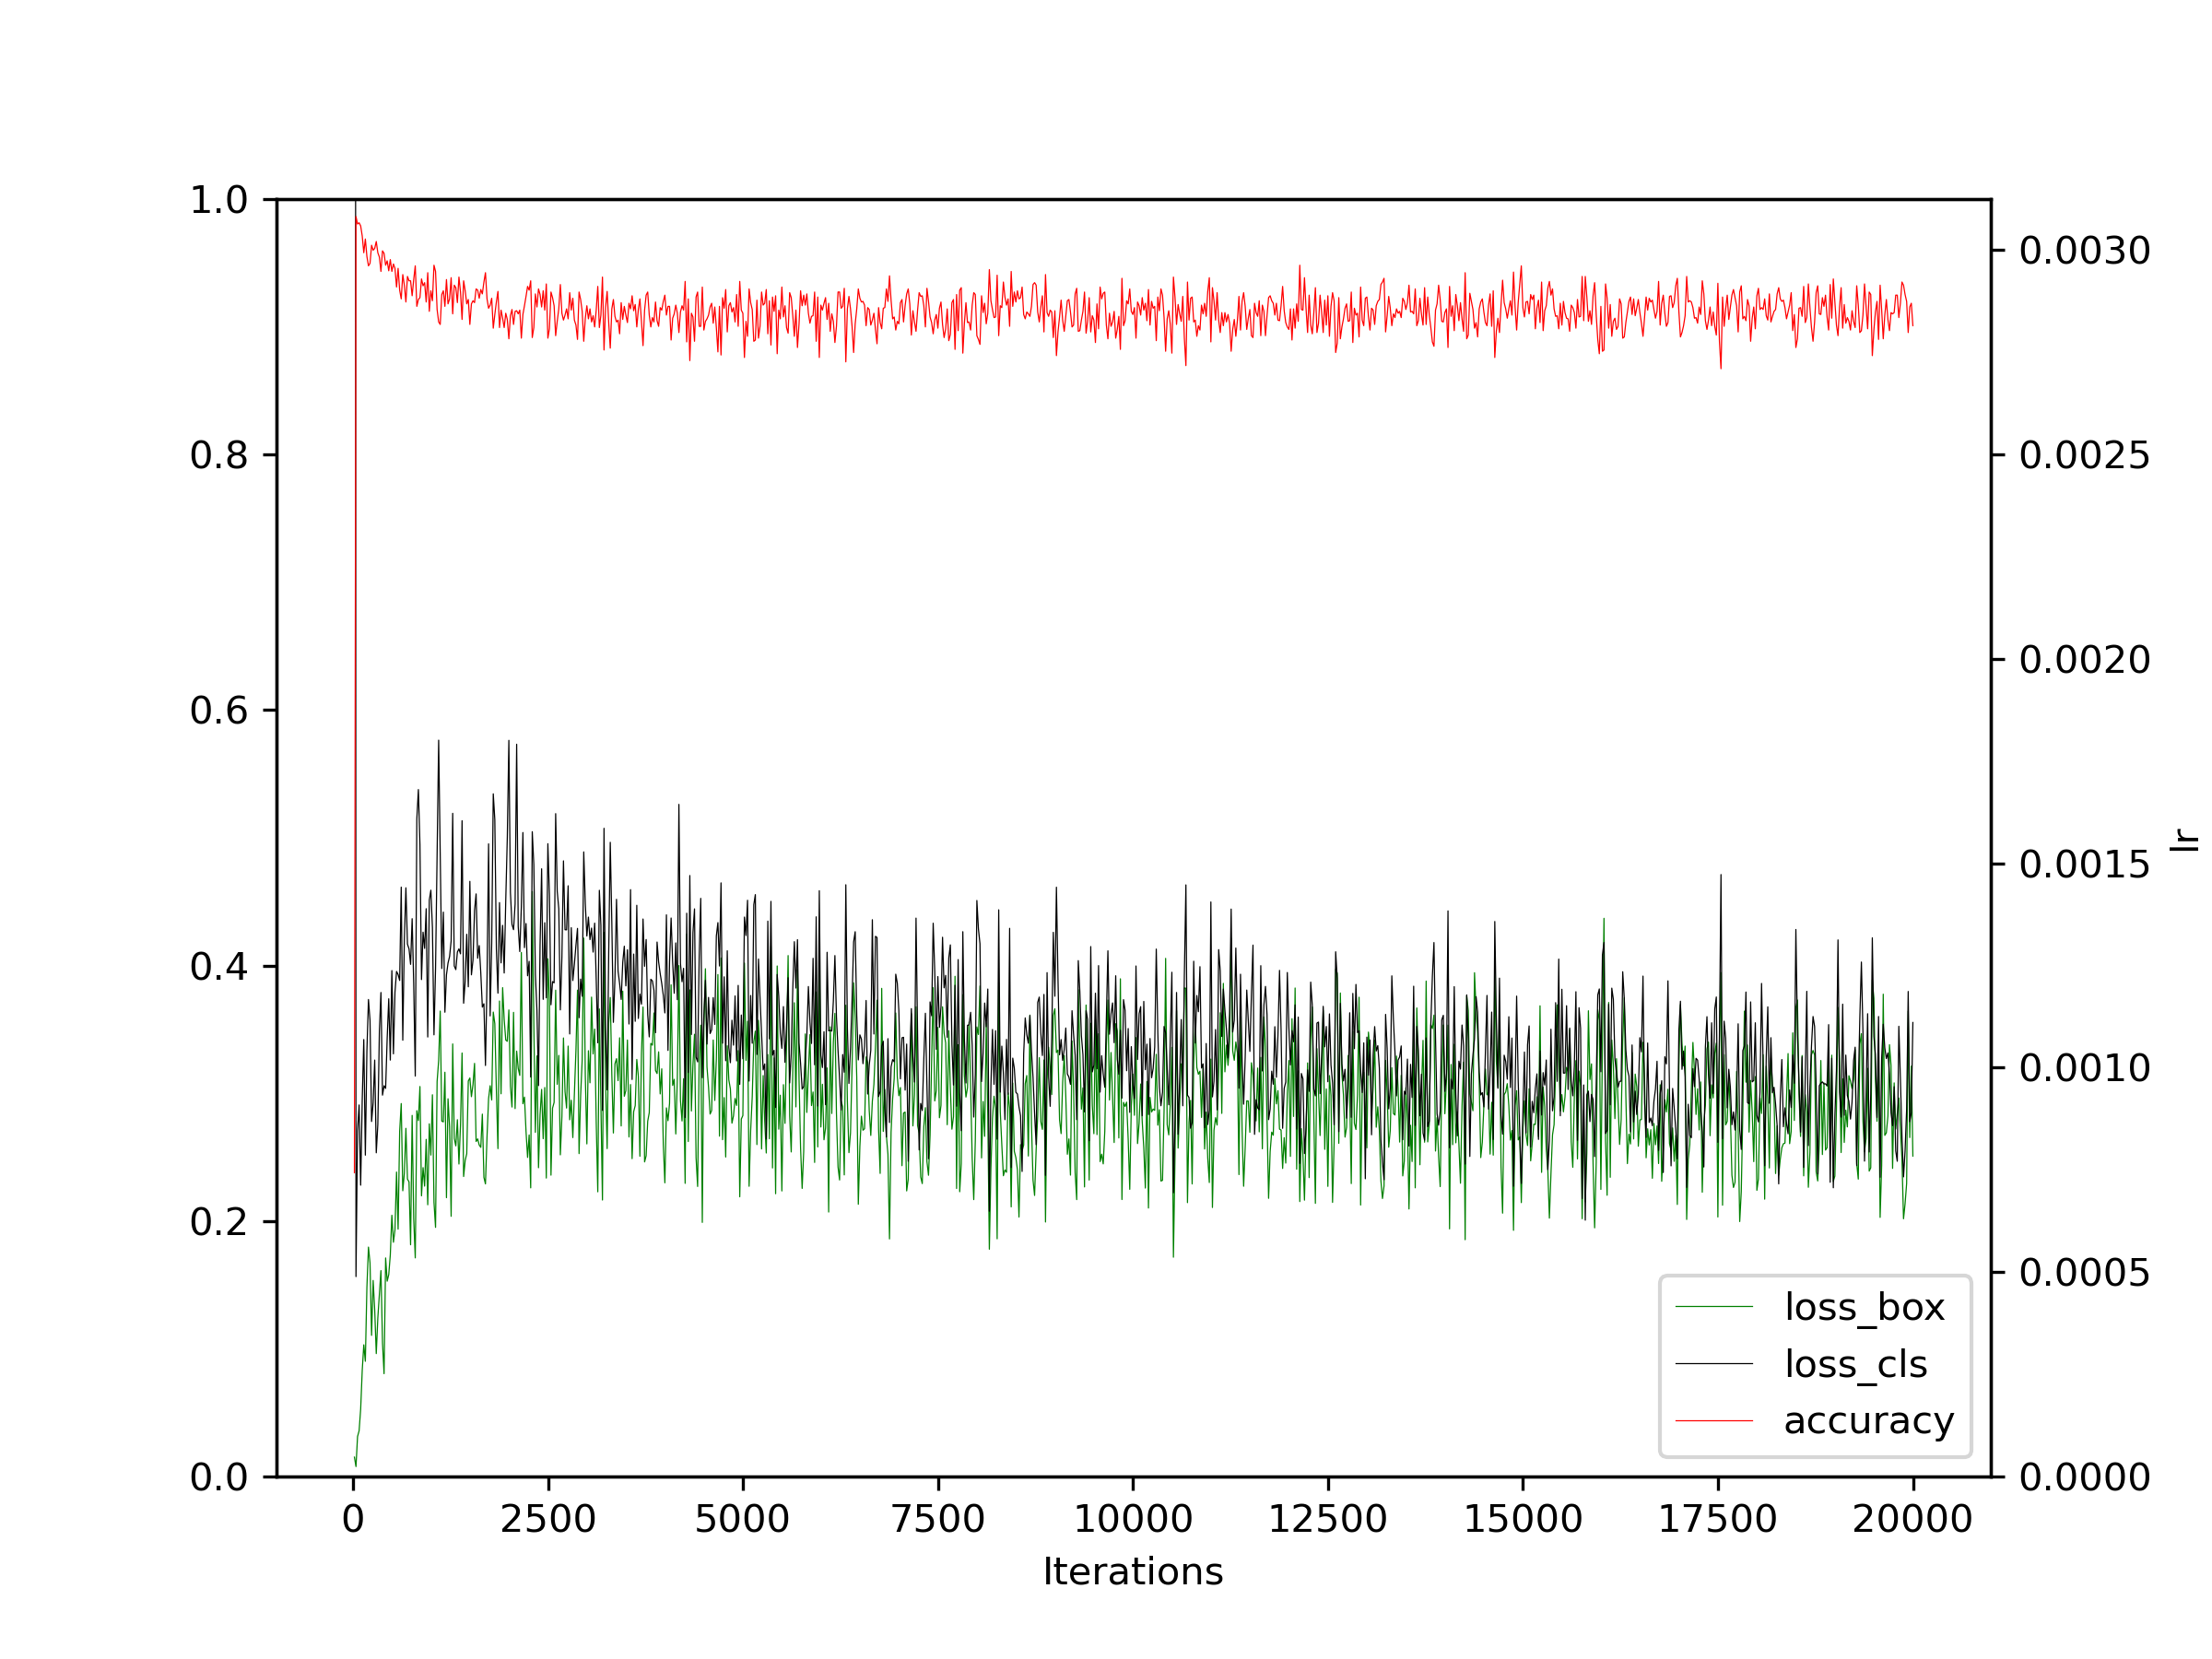
\includegraphics[width=1\textwidth]{figures/mask_rcnn_r_50_fapn_1x_20000iter.png}
    \caption{Mask RCNN \& FaPN with 20000 interactions}\label{mask_rcnn_r_50_fapn_1x_20000iter}
\end{figure}


It can be seen that after 20000 iterations and default parameter training, the accuracy rate has stabilized at the level of 95\%, and both loss box and loss cls are proficient to within 0.002, with sufficient performance for use.


Then Faster RCNN \cite{ren2015faster} was trained on 10,000 iterations after adding the FaPN module, and the results shown in the figure below were obtained.

% \begin{figure}[htb]
%     \centering
%     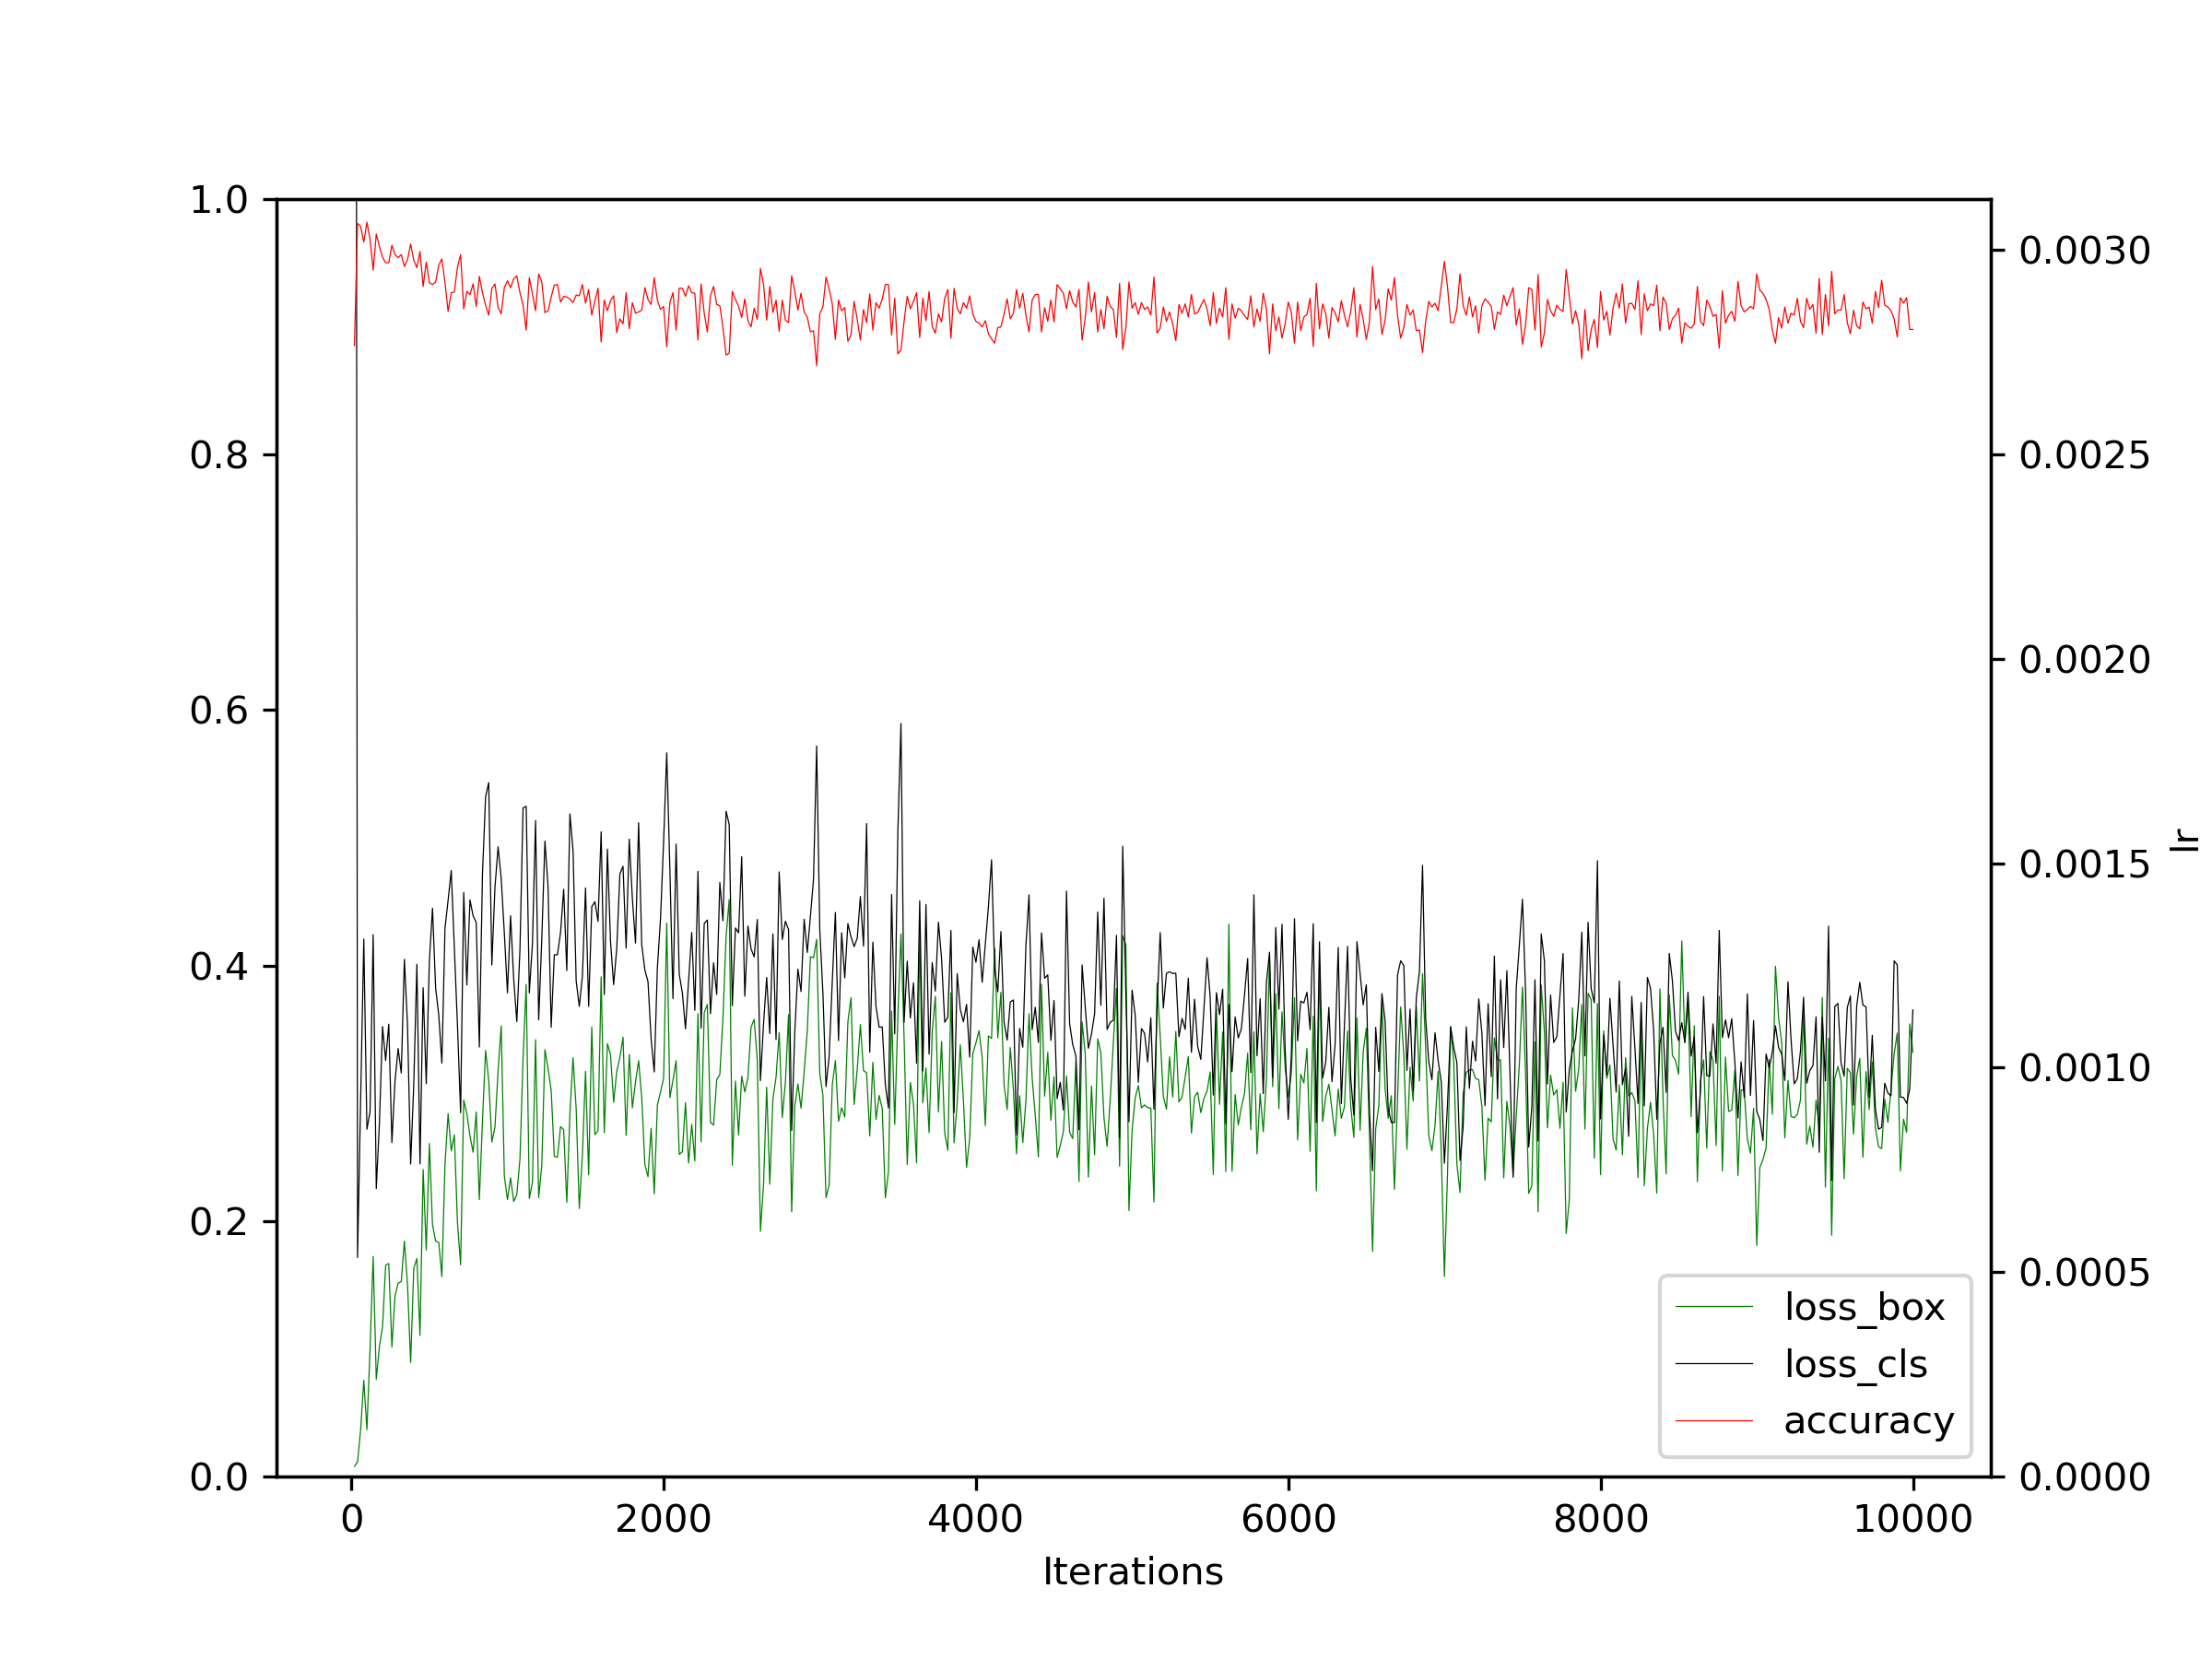
\includegraphics[width=1\textwidth]{figures/faster_rcnn_r_50_fapn_1x_10000iter.png}
%     \caption{Faster RCNN \& FaPN with 10000 interactions}\label{faster_rcnn_r_50_fapn_1x_10000iter}
% \end{figure}


It can be seen that whether Mask RCNN \cite{he2017mask} or Faster RCNN plus FaPN is used for training on the COCO2017 dataset, higher accuracy and better performance can be obtained under 10,000 iterations, and it has strong practicability.


\begin{table}[htb]
% h-here,t-top,b-bottom,优先级依次下降
    \begin{center}
    % 居中
        \caption{Performance of the Faster RCNN on category pedestrian}\label{table1}
        \begin{tabular}{|c|c|c|c|c|c|c|} % 三线表不能有竖线,l-left,c-center,r-right
            \toprule
            %三线表-top 线
            \textbf{Method} & \textbf{Backbone}&\textbf{Iterations} & $AP$ & $AP_s$ & $AP_m$ & $AP_l$ \\
            \hline
            %三线表-middle 线
            FaPN          & \multirow{5}{*}{Faster R-CNN R50}&10K &10.1&5.3&11.4&11.9 \\
            FaPN          &  &20K&12.6&9.5&12.8&15.7 \\
			FaPN (fully trained)         & &65K &40.2&23.9&43.9&48.8 \\
			FaPN (authors')         &  &-&39.2&24.5&43.3&49.1 \\
			FPN  & &- &37.9&22.4&41.1&49.1 \\
            \bottomrule
            %三线表-底线
        \end{tabular}
    \end{center}
\end{table}

\begin{table}[htb]
	% h-here,t-top,b-bottom,优先级依次下降
		\begin{center}
		% 居中
			\caption{Performance of the Mask RCNN on category pedestrian}\label{table2}
			\begin{tabular}{|c|c|c|c|c|c} % 三线表不能有竖线,l-left,c-center,r-right
				\toprule
				%三线表-top 线
				\textbf{Method} & \textbf{Backbone}&\textbf{Iterations} & $AP^{mask}$ & $AP^{mask}_s$ \\
				\hline
				%三线表-middle 线
				FaPN & \multirow{5}{*}{Mask R-CNN R50}&10K&9.5&4.0 \\
				FaPN & &20K&14.4&5.9 \\
				FaPN (fully trained) & &80K &37.2&18.3 \\
				FaPN (authors') & &- &36.4&18.1 \\
				FPN & &- &35.2&17.1 \\
				\bottomrule
				%三线表-底线
			\end{tabular}
		\end{center}
	\end{table}


\subsection{Model Deployment}


For a trained model, we can get its checkpoint (.pth) file, which holds all the parameters of the model. If we need to deploy or evaluate a trained model, we only need to use the checkpoint file of the corresponding model.


For the server-side, we need a communication module. The function of this module is to receive the front-end data and complete the processing, call the corresponding model to complete the semantic segmentation of the image, and finally return the segmented image to the client.


The server-side adopts the socket server framework, and its basic idea is to monitor the specified port of the server. After receiving the connection request from the client, it makes a handshake with it to establish a connection. Then receive and process the relevant information and call the model.




\clearpage